\documentclass{article}
\usepackage[T1]{fontenc}
\usepackage{lmodern}
\usepackage{graphicx}
\usepackage{amsmath,amssymb}
\usepackage[a4paper,margin=2cm]{geometry}
\usepackage[absolute,overlay]{textpos}
\setlength{\TPHorizModule}{1mm}
\setlength{\TPVertModule}{1mm}
\usepackage[indonesian]{babel}
\usepackage{hyperref}
\setlength{\emergencystretch}{2em}
% unit: Halaman 18

\begin{document}

% === Halaman 18 (python/native) ===

Perfect Secrecy 

• Perfect secrecy: Cipherteks tidak menyediakan informasi apapun tentang 

   plainteks maupun kunci.

• Pada tahun 1949, Claude Shannon dari Laboratorium Bell membuktikan bahwa OTP  

memiliki perfect secrecy. Ia menulis pembuktian tsb di dalam makalahnya:

     “Shannon, C. E. (1949). Communication theory of secrecy systems. Bell System   

Technical Journal, 28(4), 656–715.”

• Menurut Shannon, suatu sistem memiliki perfect secrecy apabila setelah penyerang 

memperoleh cipherteks, informasi mengenai plainteks tidak bertambah. Secara 

matematis, kondisi tersebut dinyatakan sebagai: 

                              P(P = p ∣ C = c) = P(P = p) 

    Artinya, probabilitas suatu plainteks tertentu tetap sama sebelum maupun setelah 

cipherteks diamati

Claude Shannon

18

% deskripsi: gambar native xref 96
\noindent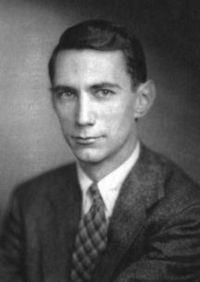
\includegraphics[width=0.85\textwidth]{../../images/python/page_018_img_01.jpeg}

\end{document}
